\section{keyboard\_\-key Class Reference}
\label{classkeyboard__key}\index{keyboard_key@{keyboard\_\-key}}
{\tt \#include $<$keyboard\_\-key.h$>$}



\subsection{Detailed Description}
\begin{Desc}
\item[Author:]root \end{Desc}




Definition at line 29 of file keyboard\_\-key.h.\subsection*{Public Types}
\begin{CompactItemize}
\item 
enum {\bf KEY\_\-TYPE} \{ {\bf KEY}, 
{\bf CHANGE}, 
{\bf ENTER}, 
{\bf BACKSPACE}
 \}
\end{CompactItemize}
\subsection*{Public Slots}
\begin{CompactItemize}
\item 
void {\bf slot\-Set\-Case} (bool {\bf upper})
\item 
void {\bf slot\-Clicked} ()
\item 
void {\bf slot\-Pressed} ()
\item 
void {\bf slot\-Released} ()
\item 
void {\bf slot\-Enter} ()
\item 
void {\bf slot\-Change} ()
\item 
void {\bf slot\-Back\-Space} ()
\item 
void {\bf slot\-Set\-Pixmap} (QPixmap,QPixmap)
\end{CompactItemize}
\subsection*{Signals}
\begin{CompactItemize}
\item 
void {\bf signal\-Send\-Char} (QString str\-Char)
\item 
void {\bf signal\-Enter} ()
\item 
void {\bf signal\-Change} ()
\item 
void {\bf signal\-Back\-Space} ()
\end{CompactItemize}
\subsection*{Public Member Functions}
\begin{CompactItemize}
\item 
{\bf keyboard\_\-key} ({\bf QWidget} $\ast$parent=0, const char $\ast$name=0, QString str\-Upper=0, QString str\-Lower=0, {\bf KEY\_\-TYPE} \_\-type=KEY)
\item 
{\bf $\sim$keyboard\_\-key} ()
\item 
void {\bf x\-Setup} (QString u, QString l)
\end{CompactItemize}
\subsection*{Protected Member Functions}
\begin{CompactItemize}
\item 
void {\bf draw\-Button} (QPainter $\ast$p)
\end{CompactItemize}
\subsection*{Private Attributes}
\begin{CompactItemize}
\item 
QString {\bf str\-Cur\-Char}
\item 
QString {\bf str\-Char\-Up}
\item 
QString {\bf str\-Char\-Lower}
\item 
bool {\bf upper}
\item 
QPixmap {\bf pix\-Background}
\item 
QPixmap {\bf pix\-Acitve}
\item 
QPixmap {\bf pix\-Inactive}
\item 
{\bf KEY\_\-TYPE} {\bf key\_\-type}
\end{CompactItemize}


\subsection{Member Enumeration Documentation}
\index{keyboard_key@{keyboard\_\-key}!KEY_TYPE@{KEY\_\-TYPE}}
\index{KEY_TYPE@{KEY\_\-TYPE}!keyboard_key@{keyboard\_\-key}}
\subsubsection{\setlength{\rightskip}{0pt plus 5cm}enum {\bf keyboard\_\-key::KEY\_\-TYPE}}\label{classkeyboard__key_keyboard__keyw4}


\begin{Desc}
\item[Enumeration values: ]\par
\begin{description}
\index{KEY@{KEY}!keyboard_key@{keyboard\_\-key}}\index{keyboard_key@{keyboard\_\-key}!KEY@{KEY}}\item[{\em 
KEY\label{classkeyboard__key_keyboard__keyw4keyboard__keyw0}
}]\index{CHANGE@{CHANGE}!keyboard_key@{keyboard\_\-key}}\index{keyboard_key@{keyboard\_\-key}!CHANGE@{CHANGE}}\item[{\em 
CHANGE\label{classkeyboard__key_keyboard__keyw4keyboard__keyw1}
}]\index{ENTER@{ENTER}!keyboard_key@{keyboard\_\-key}}\index{keyboard_key@{keyboard\_\-key}!ENTER@{ENTER}}\item[{\em 
ENTER\label{classkeyboard__key_keyboard__keyw4keyboard__keyw2}
}]\index{BACKSPACE@{BACKSPACE}!keyboard_key@{keyboard\_\-key}}\index{keyboard_key@{keyboard\_\-key}!BACKSPACE@{BACKSPACE}}\item[{\em 
BACKSPACE\label{classkeyboard__key_keyboard__keyw4keyboard__keyw3}
}]\end{description}
\end{Desc}



Definition at line 34 of file keyboard\_\-key.h.



\footnotesize\begin{verbatim}35 {
36   KEY,
37   CHANGE,
38   ENTER,
39   BACKSPACE
40 };
\end{verbatim}\normalsize 


\subsection{Constructor \& Destructor Documentation}
\index{keyboard_key@{keyboard\_\-key}!keyboard_key@{keyboard\_\-key}}
\index{keyboard_key@{keyboard\_\-key}!keyboard_key@{keyboard\_\-key}}
\subsubsection{\setlength{\rightskip}{0pt plus 5cm}keyboard\_\-key::keyboard\_\-key ({\bf QWidget} $\ast$ {\em parent} = 0, const char $\ast$ {\em name} = 0, QString {\em str\-Upper} = 0, QString {\em str\-Lower} = 0, {\bf KEY\_\-TYPE} {\em \_\-type} = KEY)}\label{classkeyboard__key_keyboard__keya0}




Definition at line 23 of file keyboard\_\-key.cpp.

References key\_\-type, and x\-Setup().



\footnotesize\begin{verbatim}24  : QPushButton(parent, name)
25 {
26    
27    key_type=_type;
28    xSetup(strUpper,strLower);
29 }
\end{verbatim}\normalsize 


Here is the call graph for this function:\begin{figure}[H]
\begin{center}
\leavevmode
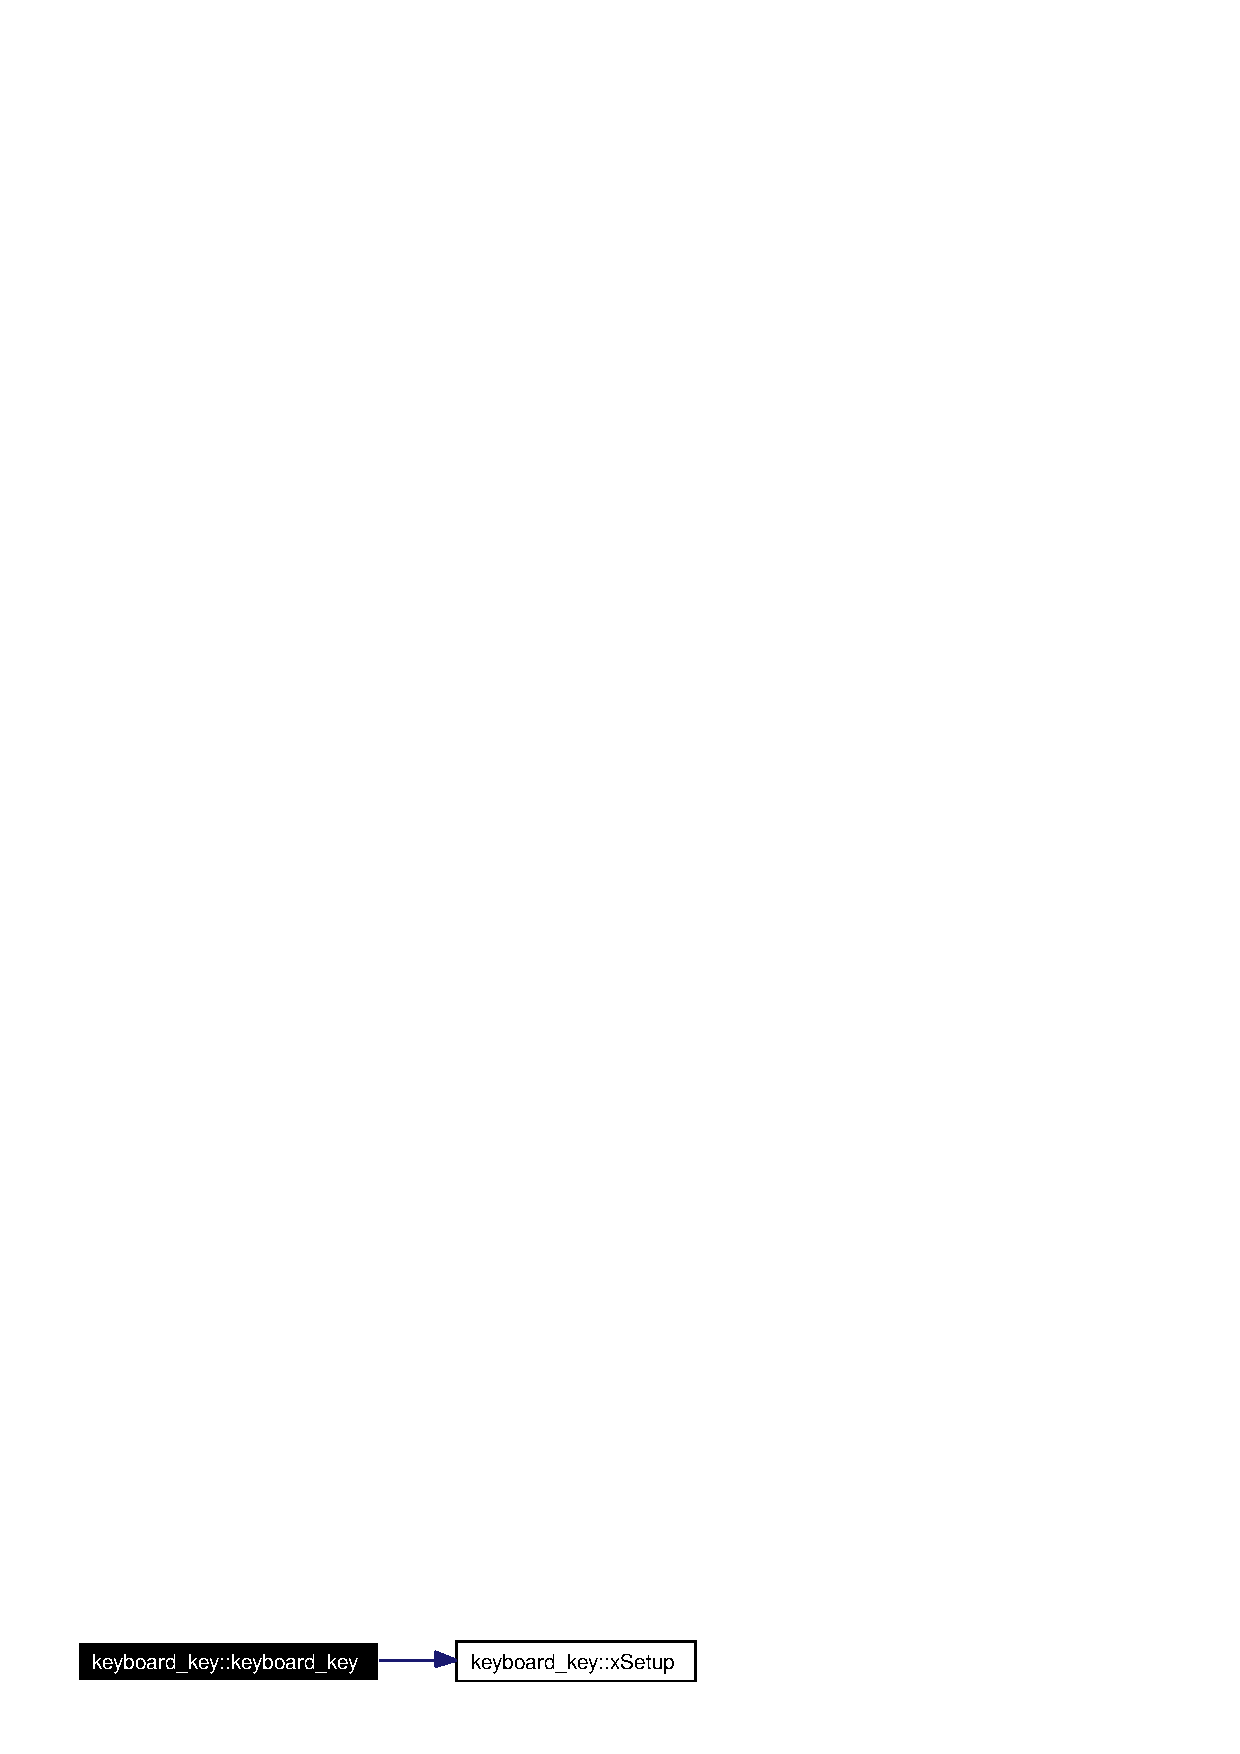
\includegraphics[width=167pt]{classkeyboard__key_keyboard__keya0_cgraph}
\end{center}
\end{figure}
\index{keyboard_key@{keyboard\_\-key}!~keyboard_key@{$\sim$keyboard\_\-key}}
\index{~keyboard_key@{$\sim$keyboard\_\-key}!keyboard_key@{keyboard\_\-key}}
\subsubsection{\setlength{\rightskip}{0pt plus 5cm}keyboard\_\-key::$\sim${\bf keyboard\_\-key} ()}\label{classkeyboard__key_keyboard__keya1}




Definition at line 32 of file keyboard\_\-key.cpp.



\footnotesize\begin{verbatim}33 {
34 }
\end{verbatim}\normalsize 


\subsection{Member Function Documentation}
\index{keyboard_key@{keyboard\_\-key}!drawButton@{drawButton}}
\index{drawButton@{drawButton}!keyboard_key@{keyboard\_\-key}}
\subsubsection{\setlength{\rightskip}{0pt plus 5cm}void keyboard\_\-key::draw\-Button (QPainter $\ast$ {\em p})\hspace{0.3cm}{\tt  [protected]}}\label{classkeyboard__key_keyboard__keyb0}




Definition at line 91 of file keyboard\_\-key.cpp.

References str\-Cur\-Char.



\footnotesize\begin{verbatim}92 {
93   p->drawPixmap(0,0,pixBackground);
94   p->drawText( rect(), AlignCenter, strCurChar );
95 }
\end{verbatim}\normalsize 
\index{keyboard_key@{keyboard\_\-key}!signalBackSpace@{signalBackSpace}}
\index{signalBackSpace@{signalBackSpace}!keyboard_key@{keyboard\_\-key}}
\subsubsection{\setlength{\rightskip}{0pt plus 5cm}void keyboard\_\-key::signal\-Back\-Space ()\hspace{0.3cm}{\tt  [signal]}}\label{classkeyboard__key_keyboard__keyl3}




Definition at line 132 of file keyboard\_\-key.moc.

Referenced by slot\-Back\-Space().



\footnotesize\begin{verbatim}133 {
134     activate_signal( staticMetaObject()->signalOffset() + 3 );
135 }
\end{verbatim}\normalsize 
\index{keyboard_key@{keyboard\_\-key}!signalChange@{signalChange}}
\index{signalChange@{signalChange}!keyboard_key@{keyboard\_\-key}}
\subsubsection{\setlength{\rightskip}{0pt plus 5cm}void keyboard\_\-key::signal\-Change ()\hspace{0.3cm}{\tt  [signal]}}\label{classkeyboard__key_keyboard__keyl2}




Definition at line 126 of file keyboard\_\-key.moc.

Referenced by slot\-Change().



\footnotesize\begin{verbatim}127 {
128     activate_signal( staticMetaObject()->signalOffset() + 2 );
129 }
\end{verbatim}\normalsize 
\index{keyboard_key@{keyboard\_\-key}!signalEnter@{signalEnter}}
\index{signalEnter@{signalEnter}!keyboard_key@{keyboard\_\-key}}
\subsubsection{\setlength{\rightskip}{0pt plus 5cm}void keyboard\_\-key::signal\-Enter ()\hspace{0.3cm}{\tt  [signal]}}\label{classkeyboard__key_keyboard__keyl1}




Definition at line 120 of file keyboard\_\-key.moc.

Referenced by slot\-Enter().



\footnotesize\begin{verbatim}121 {
122     activate_signal( staticMetaObject()->signalOffset() + 1 );
123 }
\end{verbatim}\normalsize 
\index{keyboard_key@{keyboard\_\-key}!signalSendChar@{signalSendChar}}
\index{signalSendChar@{signalSendChar}!keyboard_key@{keyboard\_\-key}}
\subsubsection{\setlength{\rightskip}{0pt plus 5cm}void keyboard\_\-key::signal\-Send\-Char (QString {\em str\-Char})\hspace{0.3cm}{\tt  [signal]}}\label{classkeyboard__key_keyboard__keyl0}




Definition at line 114 of file keyboard\_\-key.moc.

Referenced by slot\-Clicked().



\footnotesize\begin{verbatim}115 {
116     activate_signal( staticMetaObject()->signalOffset() + 0, t0 );
117 }
\end{verbatim}\normalsize 
\index{keyboard_key@{keyboard\_\-key}!slotBackSpace@{slotBackSpace}}
\index{slotBackSpace@{slotBackSpace}!keyboard_key@{keyboard\_\-key}}
\subsubsection{\setlength{\rightskip}{0pt plus 5cm}void keyboard\_\-key::slot\-Back\-Space ()\hspace{0.3cm}{\tt  [slot]}}\label{classkeyboard__key_keyboard__keyi6}




Definition at line 124 of file keyboard\_\-key.cpp.

References signal\-Back\-Space().

Referenced by x\-Setup().



\footnotesize\begin{verbatim}125 {
126  emit signalBackSpace();
127 }
\end{verbatim}\normalsize 
\index{keyboard_key@{keyboard\_\-key}!slotChange@{slotChange}}
\index{slotChange@{slotChange}!keyboard_key@{keyboard\_\-key}}
\subsubsection{\setlength{\rightskip}{0pt plus 5cm}void keyboard\_\-key::slot\-Change ()\hspace{0.3cm}{\tt  [slot]}}\label{classkeyboard__key_keyboard__keyi5}




Definition at line 119 of file keyboard\_\-key.cpp.

References signal\-Change().

Referenced by x\-Setup().



\footnotesize\begin{verbatim}120 {
121   emit signalChange();
122 }
\end{verbatim}\normalsize 
\index{keyboard_key@{keyboard\_\-key}!slotClicked@{slotClicked}}
\index{slotClicked@{slotClicked}!keyboard_key@{keyboard\_\-key}}
\subsubsection{\setlength{\rightskip}{0pt plus 5cm}void keyboard\_\-key::slot\-Clicked ()\hspace{0.3cm}{\tt  [slot]}}\label{classkeyboard__key_keyboard__keyi1}




Definition at line 86 of file keyboard\_\-key.cpp.

References signal\-Send\-Char(), and str\-Cur\-Char.

Referenced by x\-Setup().



\footnotesize\begin{verbatim}87 {
88    emit signalSendChar(strCurChar);
89 }
\end{verbatim}\normalsize 
\index{keyboard_key@{keyboard\_\-key}!slotEnter@{slotEnter}}
\index{slotEnter@{slotEnter}!keyboard_key@{keyboard\_\-key}}
\subsubsection{\setlength{\rightskip}{0pt plus 5cm}void keyboard\_\-key::slot\-Enter ()\hspace{0.3cm}{\tt  [slot]}}\label{classkeyboard__key_keyboard__keyi4}




Definition at line 114 of file keyboard\_\-key.cpp.

References signal\-Enter().

Referenced by x\-Setup().



\footnotesize\begin{verbatim}115 {
116   emit signalEnter();
117 }
\end{verbatim}\normalsize 
\index{keyboard_key@{keyboard\_\-key}!slotPressed@{slotPressed}}
\index{slotPressed@{slotPressed}!keyboard_key@{keyboard\_\-key}}
\subsubsection{\setlength{\rightskip}{0pt plus 5cm}void keyboard\_\-key::slot\-Pressed ()\hspace{0.3cm}{\tt  [slot]}}\label{classkeyboard__key_keyboard__keyi2}




Definition at line 96 of file keyboard\_\-key.cpp.

References pix\-Acitve.

Referenced by x\-Setup().



\footnotesize\begin{verbatim}97 {
98   pixBackground=pixAcitve;
99   repaint();
100 }
\end{verbatim}\normalsize 
\index{keyboard_key@{keyboard\_\-key}!slotReleased@{slotReleased}}
\index{slotReleased@{slotReleased}!keyboard_key@{keyboard\_\-key}}
\subsubsection{\setlength{\rightskip}{0pt plus 5cm}void keyboard\_\-key::slot\-Released ()\hspace{0.3cm}{\tt  [slot]}}\label{classkeyboard__key_keyboard__keyi3}




Definition at line 101 of file keyboard\_\-key.cpp.

References pix\-Inactive.

Referenced by x\-Setup().



\footnotesize\begin{verbatim}102 {
103  pixBackground=pixInactive;
104  repaint();
105 }
\end{verbatim}\normalsize 
\index{keyboard_key@{keyboard\_\-key}!slotSetCase@{slotSetCase}}
\index{slotSetCase@{slotSetCase}!keyboard_key@{keyboard\_\-key}}
\subsubsection{\setlength{\rightskip}{0pt plus 5cm}void keyboard\_\-key::slot\-Set\-Case (bool {\em upper})\hspace{0.3cm}{\tt  [slot]}}\label{classkeyboard__key_keyboard__keyi0}




Definition at line 77 of file keyboard\_\-key.cpp.

References str\-Char\-Lower, str\-Char\-Up, and str\-Cur\-Char.

Referenced by x\-Setup().



\footnotesize\begin{verbatim}78 {
79    if(upper)
80    strCurChar=strCharUp;
81    else
82    strCurChar=strCharLower;
83    repaint();
84 }
\end{verbatim}\normalsize 
\index{keyboard_key@{keyboard\_\-key}!slotSetPixmap@{slotSetPixmap}}
\index{slotSetPixmap@{slotSetPixmap}!keyboard_key@{keyboard\_\-key}}
\subsubsection{\setlength{\rightskip}{0pt plus 5cm}void keyboard\_\-key::slot\-Set\-Pixmap (QPixmap, QPixmap)\hspace{0.3cm}{\tt  [slot]}}\label{classkeyboard__key_keyboard__keyi7}




Definition at line 106 of file keyboard\_\-key.cpp.

References pix\-Acitve, and pix\-Inactive.

Referenced by keyboard::Init\-Key().



\footnotesize\begin{verbatim}107 {
108    pixInactive=inactive;
109    pixAcitve=pix_active;
110    pixBackground=pixInactive;
111    resize(pixBackground.size());
112    repaint();
113 }
\end{verbatim}\normalsize 
\index{keyboard_key@{keyboard\_\-key}!xSetup@{xSetup}}
\index{xSetup@{xSetup}!keyboard_key@{keyboard\_\-key}}
\subsubsection{\setlength{\rightskip}{0pt plus 5cm}void keyboard\_\-key::x\-Setup (QString {\em u}, QString {\em l})}\label{classkeyboard__key_keyboard__keya2}




Definition at line 35 of file keyboard\_\-key.cpp.

References BACKSPACE, CHANGE, ENTER, KEY, key\_\-type, pix\-Acitve, pix\-Inactive, slot\-Back\-Space(), slot\-Change(), slot\-Clicked(), slot\-Enter(), slot\-Pressed(), slot\-Released(), slot\-Set\-Case(), str\-Char\-Lower, and str\-Char\-Up.

Referenced by keyboard\_\-key().



\footnotesize\begin{verbatim}36 { 
37   //DAVID  set up
38   pixInactive.load("/root/kde_application/hdass08/skin/keybtn.png");
39   pixAcitve.load("/root/kde_application/hdass08/skin/keybtn-active.png");
40   pixBackground=pixInactive;
41   //QBitmap mask=QBitmap("/root/kde_application/hdass08/skin/key_btn_mask.png");
42   //setMask(mask);
43   resize(pixBackground.size());
44   QFont serifFont( "Helvetica", 18, QFont::Bold );
45   setFont(serifFont); 
46   strCharUp=up;
47   strCharLower=lo;
48   //DAVID default is the lowercase
49   upper=true;
50   slotSetCase(upper);
51   //setText(strCharLower);
52   switch(key_type)
53   {
54    case KEY:
55    
56    connect(this,SIGNAL(clicked()),this,SLOT(slotClicked()));
57    break;
58    
59    case ENTER:
60    
61    connect(this,SIGNAL(clicked()),this,SLOT(slotEnter()));
62    break;
63    
64    case BACKSPACE:
65    connect(this,SIGNAL(clicked()),this,SLOT(slotBackSpace()));
66    break;  
67    
68    case CHANGE:
69    connect(this,SIGNAL(clicked()),this,SLOT(slotChange()));
70    break; 
71   }
72   
73   connect(this,SIGNAL(pressed()),this,SLOT(slotPressed()));
74   connect(this,SIGNAL(released()),this,SLOT(slotReleased()));
75 }
\end{verbatim}\normalsize 


\subsection{Member Data Documentation}
\index{keyboard_key@{keyboard\_\-key}!key_type@{key\_\-type}}
\index{key_type@{key\_\-type}!keyboard_key@{keyboard\_\-key}}
\subsubsection{\setlength{\rightskip}{0pt plus 5cm}{\bf KEY\_\-TYPE} {\bf keyboard\_\-key::key\_\-type}\hspace{0.3cm}{\tt  [private]}}\label{classkeyboard__key_keyboard__keyr7}




Definition at line 66 of file keyboard\_\-key.h.

Referenced by keyboard\_\-key(), and x\-Setup().\index{keyboard_key@{keyboard\_\-key}!pixAcitve@{pixAcitve}}
\index{pixAcitve@{pixAcitve}!keyboard_key@{keyboard\_\-key}}
\subsubsection{\setlength{\rightskip}{0pt plus 5cm}QPixmap {\bf keyboard\_\-key::pix\-Acitve}\hspace{0.3cm}{\tt  [private]}}\label{classkeyboard__key_keyboard__keyr5}




Definition at line 65 of file keyboard\_\-key.h.

Referenced by slot\-Pressed(), slot\-Set\-Pixmap(), and x\-Setup().\index{keyboard_key@{keyboard\_\-key}!pixBackground@{pixBackground}}
\index{pixBackground@{pixBackground}!keyboard_key@{keyboard\_\-key}}
\subsubsection{\setlength{\rightskip}{0pt plus 5cm}QPixmap {\bf keyboard\_\-key::pix\-Background}\hspace{0.3cm}{\tt  [private]}}\label{classkeyboard__key_keyboard__keyr4}




Definition at line 65 of file keyboard\_\-key.h.\index{keyboard_key@{keyboard\_\-key}!pixInactive@{pixInactive}}
\index{pixInactive@{pixInactive}!keyboard_key@{keyboard\_\-key}}
\subsubsection{\setlength{\rightskip}{0pt plus 5cm}QPixmap {\bf keyboard\_\-key::pix\-Inactive}\hspace{0.3cm}{\tt  [private]}}\label{classkeyboard__key_keyboard__keyr6}




Definition at line 65 of file keyboard\_\-key.h.

Referenced by slot\-Released(), slot\-Set\-Pixmap(), and x\-Setup().\index{keyboard_key@{keyboard\_\-key}!strCharLower@{strCharLower}}
\index{strCharLower@{strCharLower}!keyboard_key@{keyboard\_\-key}}
\subsubsection{\setlength{\rightskip}{0pt plus 5cm}QString {\bf keyboard\_\-key::str\-Char\-Lower}\hspace{0.3cm}{\tt  [private]}}\label{classkeyboard__key_keyboard__keyr2}




Definition at line 63 of file keyboard\_\-key.h.

Referenced by slot\-Set\-Case(), and x\-Setup().\index{keyboard_key@{keyboard\_\-key}!strCharUp@{strCharUp}}
\index{strCharUp@{strCharUp}!keyboard_key@{keyboard\_\-key}}
\subsubsection{\setlength{\rightskip}{0pt plus 5cm}QString {\bf keyboard\_\-key::str\-Char\-Up}\hspace{0.3cm}{\tt  [private]}}\label{classkeyboard__key_keyboard__keyr1}




Definition at line 63 of file keyboard\_\-key.h.

Referenced by slot\-Set\-Case(), and x\-Setup().\index{keyboard_key@{keyboard\_\-key}!strCurChar@{strCurChar}}
\index{strCurChar@{strCurChar}!keyboard_key@{keyboard\_\-key}}
\subsubsection{\setlength{\rightskip}{0pt plus 5cm}QString {\bf keyboard\_\-key::str\-Cur\-Char}\hspace{0.3cm}{\tt  [private]}}\label{classkeyboard__key_keyboard__keyr0}




Definition at line 63 of file keyboard\_\-key.h.

Referenced by draw\-Button(), slot\-Clicked(), and slot\-Set\-Case().\index{keyboard_key@{keyboard\_\-key}!upper@{upper}}
\index{upper@{upper}!keyboard_key@{keyboard\_\-key}}
\subsubsection{\setlength{\rightskip}{0pt plus 5cm}bool {\bf keyboard\_\-key::upper}\hspace{0.3cm}{\tt  [private]}}\label{classkeyboard__key_keyboard__keyr3}




Definition at line 64 of file keyboard\_\-key.h.

The documentation for this class was generated from the following files:\begin{CompactItemize}
\item 
{\bf keyboard\_\-key.h}\item 
{\bf keyboard\_\-key.moc}\item 
{\bf keyboard\_\-key.cpp}\end{CompactItemize}
